\chapter{Results}
In this section we present and compare results of the four models aplied in STLF. The performance of the models are evaluated using MAPE, MAE, RMSE and R\^2. These metrics can give us a clear picture and comparisons framework for each of the model performance.  The goal is to represent the accuracy, robustness and suitability of the ML and AI models to solve STLF.

The metrics theory is explained in \ref{sec:eval_metrics} which shows the mathematics behind each of the metrics used in the research. The methodology shows the creation of the models and how these results were produced. 


\section{Dataset Results}
 The continuous\_dataset.csv contained well ordered data that was collected with minimum errors, empty data was filled using the forward and back-filling process.Figure \ref{fig:originaldataset}
 \begin{figure}[h]
 	\centering
 \begin{minipage}[b]{0.45\linewidth}
 	\centering
 	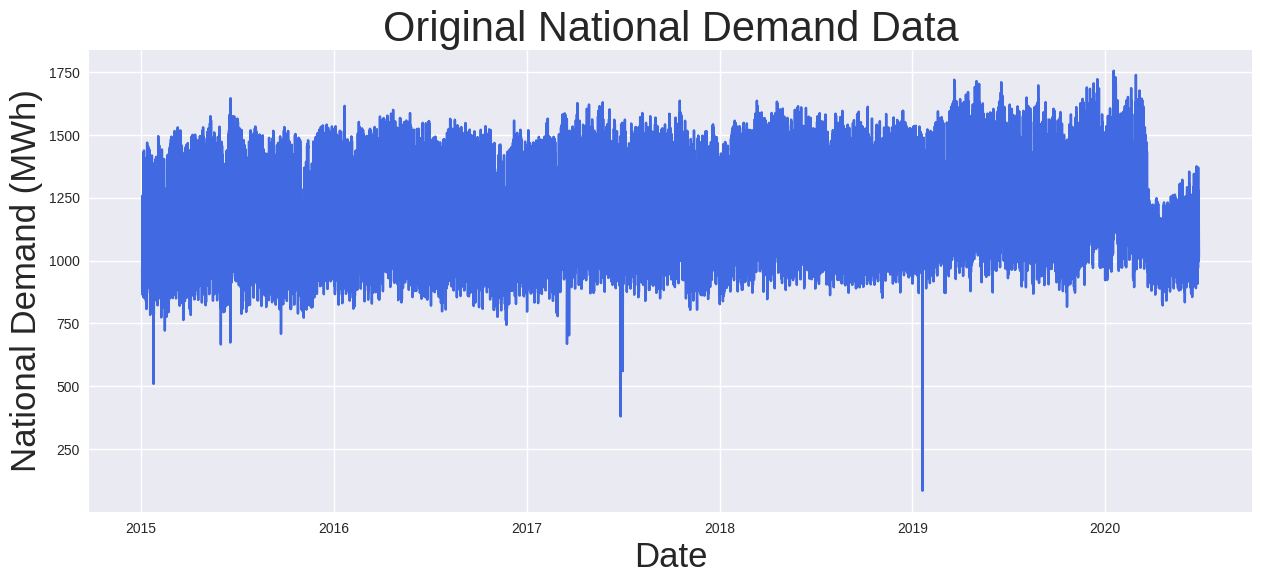
\includegraphics[width=\linewidth]{Chapters/images/results/original_dataset}
 	\caption{The original national demand .}
 	\label{fig:originaldataset}
 \end{minipage}
 \begin{minipage}[b]{0.45\linewidth}
 	\centering
 	\includegraphics[width=\linewidth]{"Chapters/images/results/train test split_after HI"}
 	\caption{HI processed dataset with traintest split.}
 	\label{fig:train-test-splitafter-hi}
 \end{minipage}
 \end{figure}
 
 The HI method explained in section \ref{sec:HI_method}, was used to handle outliers in the dataset, fixing all data-points that deviated from the normalcy presented in the dataset. After the implementation of the HI-method the train test split of 80/20 was implemented. Figure \ref{fig:train-test-splitafter-hi} shows the effectiveness of the HI method in removing noisy details in the dataset.

 \begin{figure}[h]
  	\centering
  	% First figure
  	\begin{minipage}[b]{0.45\linewidth}
  		\centering
  		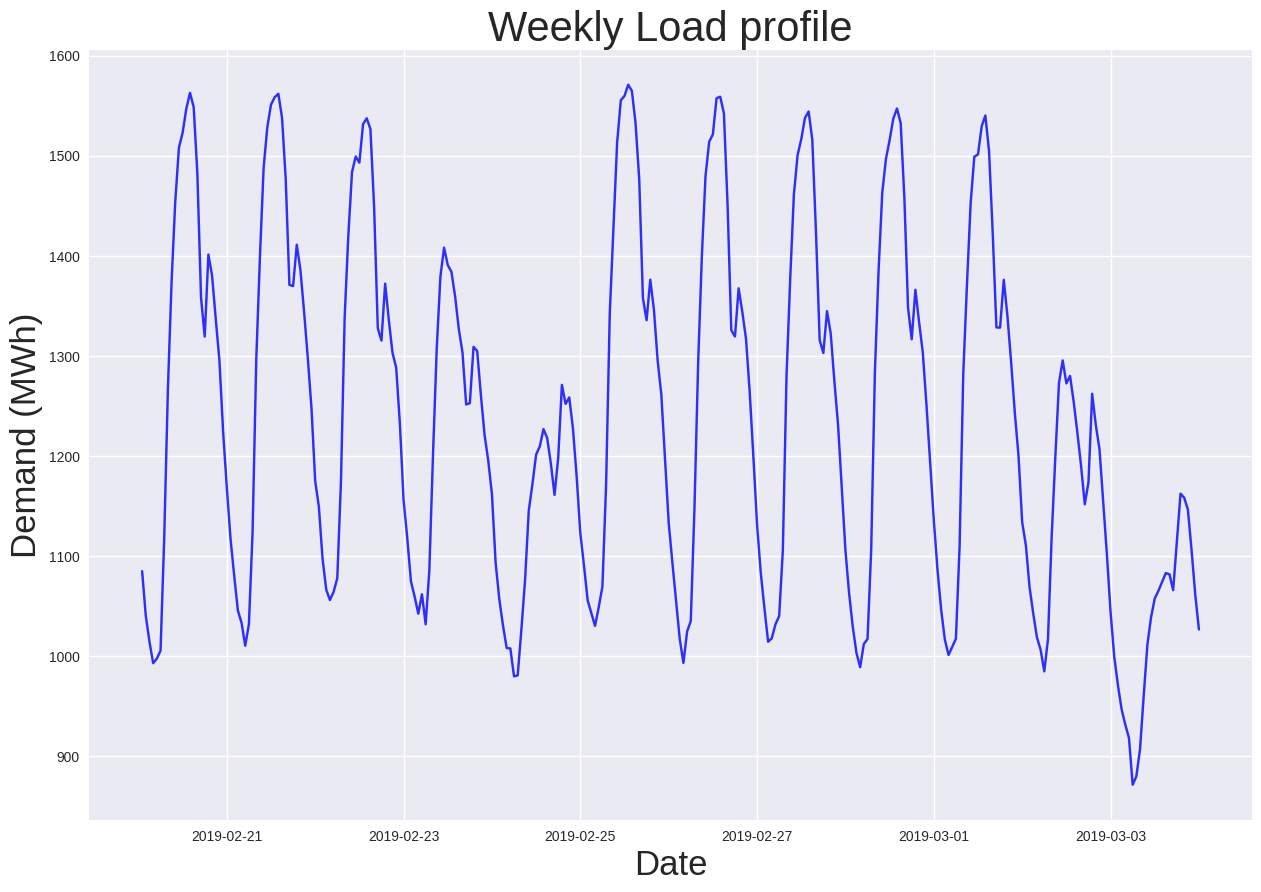
\includegraphics[width=\linewidth]{Chapters/images/results/weekly_load_profile.png}
  		\caption{The general weekly national load profile.}
  		\label{fig:weeklyloadprofile}
  	\end{minipage}
  	\hfill
  	% Second figure
  	\begin{minipage}[b]{0.45\linewidth}
  		\centering
  		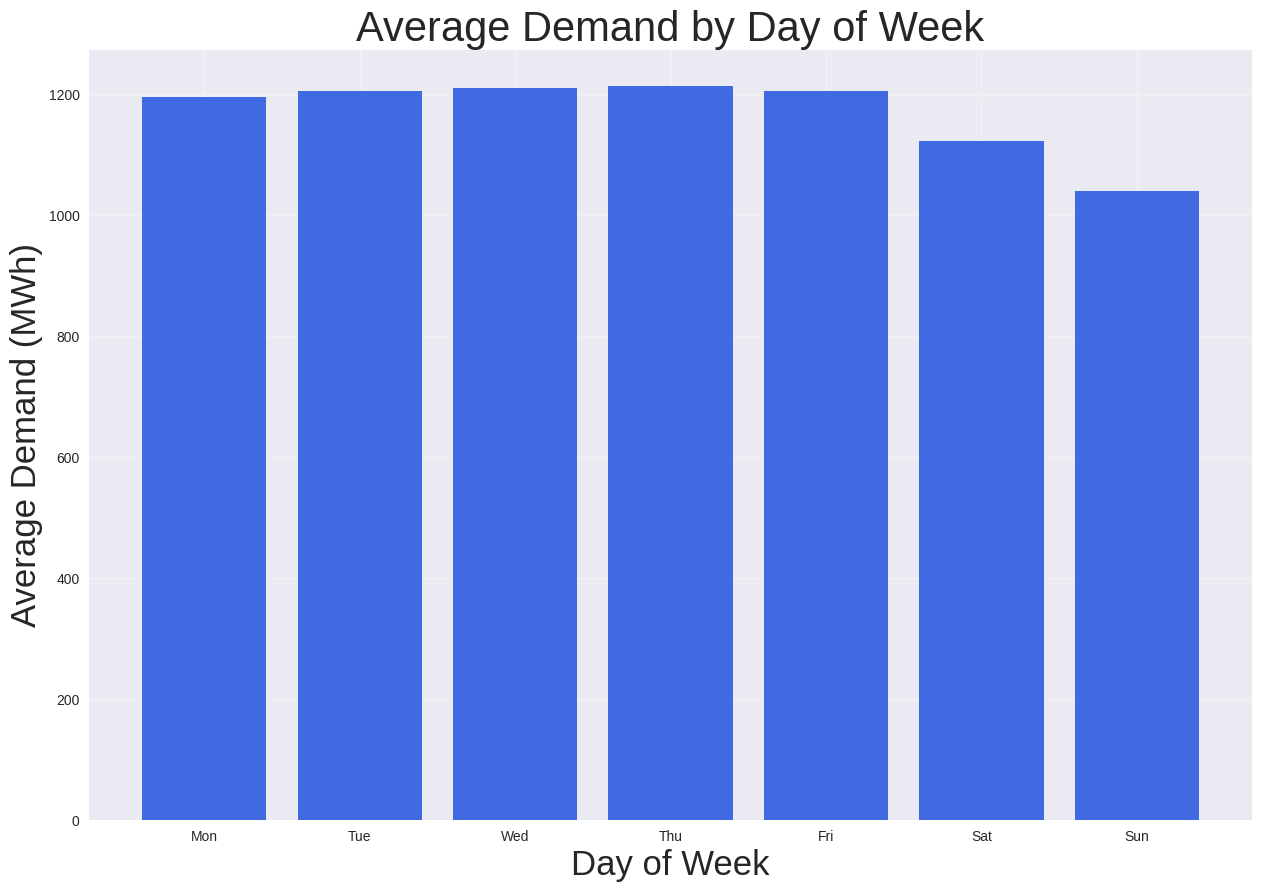
\includegraphics[width=\linewidth]{Chapters/images/results/average_daily_demand.png}
  		\caption{The weekly average daily demand }
  		\label{fig:averagedailydemand}
  	\end{minipage}
  \end{figure}
  
  
  To further understand the dataset, it was broken down to give the more insight on how the data and load behaves at different points. Firstly the weekly load profile in figure \ref{fig:weeklyloadprofile} shows a daily pattern that the load exhibits.The trend shows a higher usage during the week and lower usage in the weekend, with the lowest usage day being Sunday. 
  
  
  Figure \ref{fig:averagedailydemand} shows the average daily demand  of electricity. It also shows a higher usage during the week and lower consumption on the weekend, with Sunday being the lowest consumption day. 
  \begin{figure}[h]
  	\centering
  	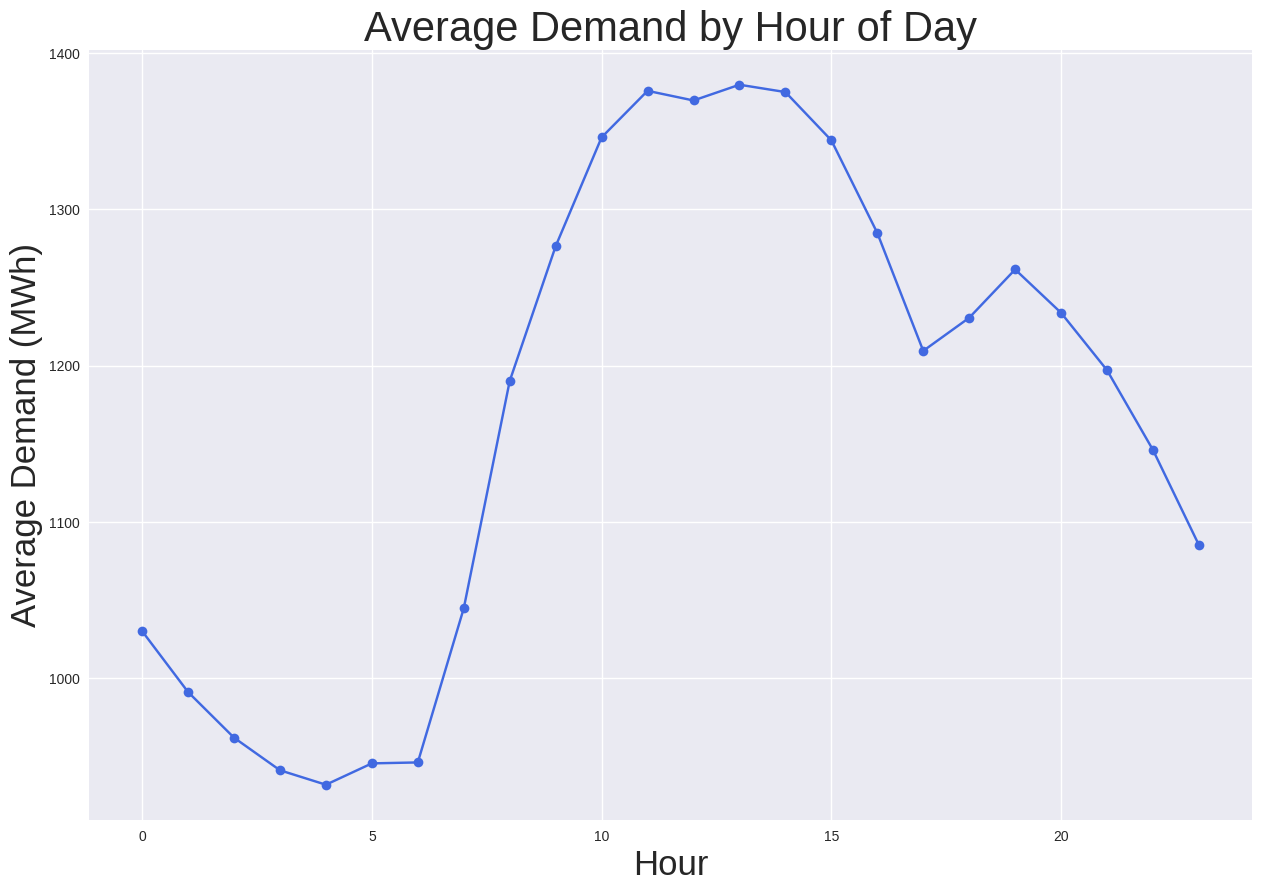
\includegraphics[width=0.45\linewidth]{Chapters/images/results/average_hourly_demand}
  	\caption{Average hourly demand of electricity between 2015 and 2020 in panama}
  	\label{fig:averagehourlydemand}
  \end{figure}
  
  Figure \ref{fig:averagehourlydemand} shows the average hourly usage of data. The averages show that the lowest consumption is in the early hours of the day, with a steady rise in the early morning leading to a peak at midday. After midday there is a steady decrease in demand with a slight increase between the 18th and 20th hour of the day, this is followed by a drop in usage leading to the early hours of the day.  


\section{Model Simulation Results}

\subsection{Exponential smoothing}
\subsubsection{Model Choice result}
The algorithm in  Appendix \ref{sec:appendixA} figure \ref{fig:exponential-smoothing-model-choice} was used to find the best model to use for the ES model.Table \ref{tab:es_model_selection} shows the different models that were tested to find the best model.

\begin{table}[ht]
	\centering
	\resizebox{\textwidth}{!}{%
		\begin{tabular}{lccccccc}
			\hline \\
			\textbf{Model} & \textbf{Trend} & \textbf{Seasonality} & \textbf{Seasonality Period} & \textbf{Damped} & \textbf{MAPE (\%)} & \textbf{MSE (MWh)} & \textbf{AIC}
			\\
			\hline
			Simple               & None  & None & –  & No  & 13.76\%  & 180.98 & 343990.96 \\
			Double               & Add   & None & –  & No  & 15.14\%  & 172.11 & 327001.68 \\
			Triple\_Add          & Add   & Add  & 24 & No  & 10.56\%  & 125.56 & 277981.02 \\
			Triple\_Mul          & Mul   & Mul  & 24 & No   & 34.48\%  & 408.23 & 272265.85 \\
			Triple\_Add\_Damped  & Add   & Add  & 24 & Yes &  9.99\%  & 120.81 & 277708.98 \\
			Triple\_Mul\_Damped  & Mul   & Mul  & 24 & Yes & 10.01\%  & 119.49 & 272266.18 \\
			\hline
		\end{tabular}%
	}
	\caption{Exponential Smoothing Models chosen for benchmarking and their performance.}
	\label{tab:es_model_selection}
\end{table}

Comparison of performance metrics through the algorithm in figure \ref{fig:exponential-smoothing-model-choice} was the Triple Multiplicative Damped algorithm with a seasonality period of 24 data points. Since the dataset is sampled hourly the seasonality was set to 24 hours. The MAPE and MSE are very close to each other with a difference of about 0.01 each. However the AIC value for  $Triple\_Mul\_Damped$ is lower than the one for $Triple\_Add\_Damped$, this showing a better model fit for  $Triple\_Mul\_Damped$. The final choice for the ES model was  $Triple\_Mul\_Damped$ and it served as a benchmark for testing performance of other models used in the experiment.
The models tested in the research were created using python and tensorflow, using google collab an cloud jupyter notebook environment for faster processing and version control through google drive. 

The ES model being the benchmark model achieved a MAPE of 9.57\% with a MAE of 118.18Mwh using the triple Multiplicative Damped model. Table \ref{tab:exp_smoothing_results} below contains the the results produced by the ES model and the parameters of the model. 
\begin{table}[h]
	\centering
	
	\begin{tabular}{ll}
		\hline
		\textbf{Metric / Parameter} & \textbf{Value} \\
		\hline
		\multicolumn{2}{l}{\textbf{Model Results}} \\
		AIC & 20118.40 \\
		MAPE &  9.57\% \\
		MAE & 118.14 \\
		RMSE & 141.84 \\
		Correlation & 0.7239\\
		\hline
		\multicolumn{2}{l}{\textbf{Model Parameters}} \\
		Smoothing Level ($\alpha$) & 1.0000 \\
		Smoothing Trend ($\beta$) & 0.0000 \\
		Smoothing Seasonal ($\gamma$) & 0.0000 \\
		Damping Trend ($\phi$) & 0.9744 \\
		Initial Level ($l_0$) & 1071.1459 \\
		Initial Trend ($b_0$) & 1.0236 \\
		Initial Seasons & [0.9093, 0.8828, 0.8638, 0.8555, 0.8682, ...] (shape = 24) \\
		Use Box-Cox & 0.0000 \\
		Lambda ($\lambda$) & None \\
		Remove Bias & 0.0000 \\
		\hline
	\end{tabular}
	\caption{Triple Multiplicative Damped Exponential Smoothing Model Parameters and Results}
	\label{tab:exp_smoothing_results}
\end{table}
These parameters produced the best results in comparison to other ES models and this was evaluated through the algorithm shown in  \ref{fig:exponential-smoothing-model-choice}. 
\begin{figure}[h]
	\begin{minipage}[b]{0.45\linewidth}
	\centering
	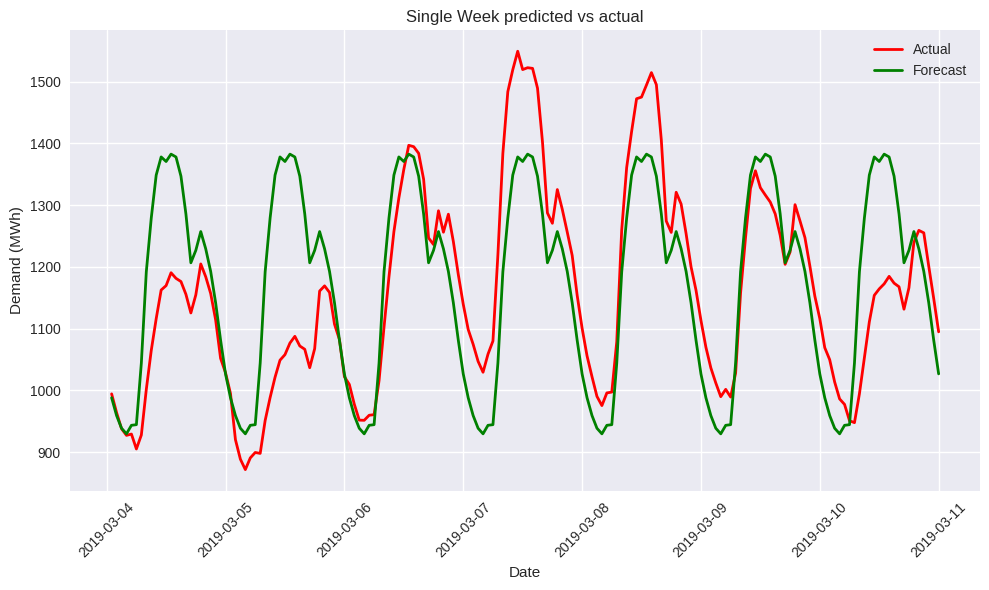
\includegraphics[width=\linewidth]{Chapters/images/results/ES_predicted_vs_actual}
	\caption{The ES predicted results against the actual demand in a week}
	\label{fig:espredictedvsactual}
\end{minipage}
\hfill
% Second figure
\begin{minipage}[b]{0.45\linewidth}
	\centering
	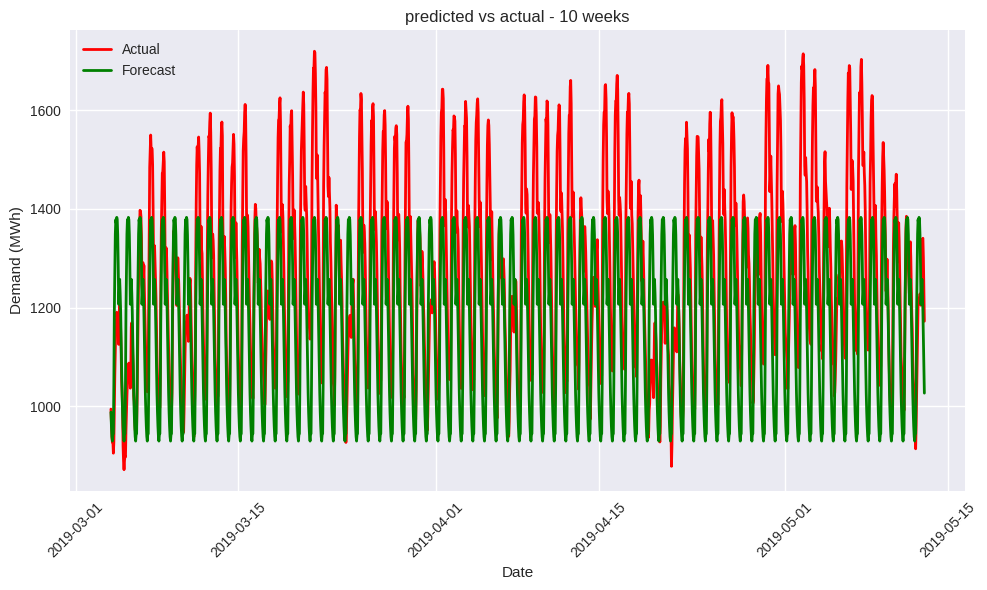
\includegraphics[width=\linewidth]{Chapters/images/results/ES_predicted_vs_actual_10weeks}
	\caption{ES model predicted vs actual load demand over 10 weeks}
	\label{fig:espredictedvsactual10weeks}
	
\end{minipage}
\end{figure}
 Figure \ref{fig:espredictedvsactual} shows the predicted and the actual values. This image shows that the model has learned the train data and does not adjust the prediction to the changing features.Figure \ref{fig:espredictedvsactual10weeks} further shows the generalization by the model. This is because ES models are not best suit for non linear problem sets.

\subsection{LSTM model results}
The LSTM model performed better than the ES model producing an MAPE value of 4.23\% and an MAE of 48.28 Mwh. LSTM models perform better because of their ability to learn context through the cell state mentioned in section \ref{sec:lstm_background}. Table \ref{tab:lstm_performance}of the results produced by the LSTM model.
\begin{table}[h]
	\centering
	
	\begin{tabular}{lc}
		\hline
		\textbf{Metric} & \textbf{Value} \\
		\hline
		Mean Squared Error (MSE) & 4548.4186 \\
		Root Mean Squared Error (RMSE) & 67.4420 \\
		Mean Absolute Error (MAE) & 48.2793 \\
		Coefficient of Determination ($R^2$) & 0.8715 \\
		Mean Absolute Percentage Error (MAPE) & 4.2312\% \\
		\hline
	\end{tabular}
	\caption{LSTM Model Performance Metrics}
	\label{tab:lstm_performance}
\end{table}
 The lower MSE and RMSE values indicate that this model has a better fit. The $R^2$ score of 0.8715 reflects a robust generalization performance and the model loss curves in figure \ref{fig:lstmmodel-loss} further show that the model is learning and generalizing properly. This image shows the decrease and stabilization of the loss values to a low value.
 \begin{figure}[h]
 	\centering
 	\includegraphics[width=0.9\linewidth]{"Chapters/images/results/lstm_model loss"}
 	\caption{The LSTM model loss during training and validation}
 	\label{fig:lstmmodel-loss}
 \end{figure}
 \textbf{Still need the prediction chart and maybe a residual plot}
 
 \subsection{DBN Model results \label{sec:dbn results}}
 The DBN model produced an impressive MAPE value of 2.13\% and an $R^2$ value of 0.966. The $R^2$ value did raise overfitting suspicions as it very high. To ensure that the model is not overfitting the train and test results were compared for the model.
 \begin{table}[h!]
 	\centering
 	\caption{Training and Testing Performance of the DBN Model}
 	\label{tab:dbn_performance}
 	\begin{tabular}{lccc}
 		\hline
 		\textbf{Metric} & \textbf{Train} & \textbf{Test} & \textbf{Difference} \\ \hline
 		MAPE (\%) & 1.6432 & 2.1264 & +0.4832 \\
 		MAE (Mwh) & 18.6358 & 26.3929 & +7.7571 \\
 		RMSE (Mwh) & 25.8889 & 34.7456 & +8.8567 \\
 		R$^2$ & 0.9819 & 0.9655 & -0.0164 \\
 		MSE & 670.2372 & 1207.2565 & +537.0193 \\ \hline
 	\end{tabular}
 \end{table}
  Table \ref{tab:dbn_performance} shows a slightly higher MAE which is expected for non seen data in the test case. The MAPE, RMSE and MSE also show an acceptable increase that represents a normal generalization in the model. The -0.016 drop in the $R^2$ value is minimal meaning that the model has not memorized the training data supporting that the model is not overfitting.
  \begin{figure}[h]
  	\centering
  	\begin{minipage}[b]{0.48\linewidth}
  		\centering
  		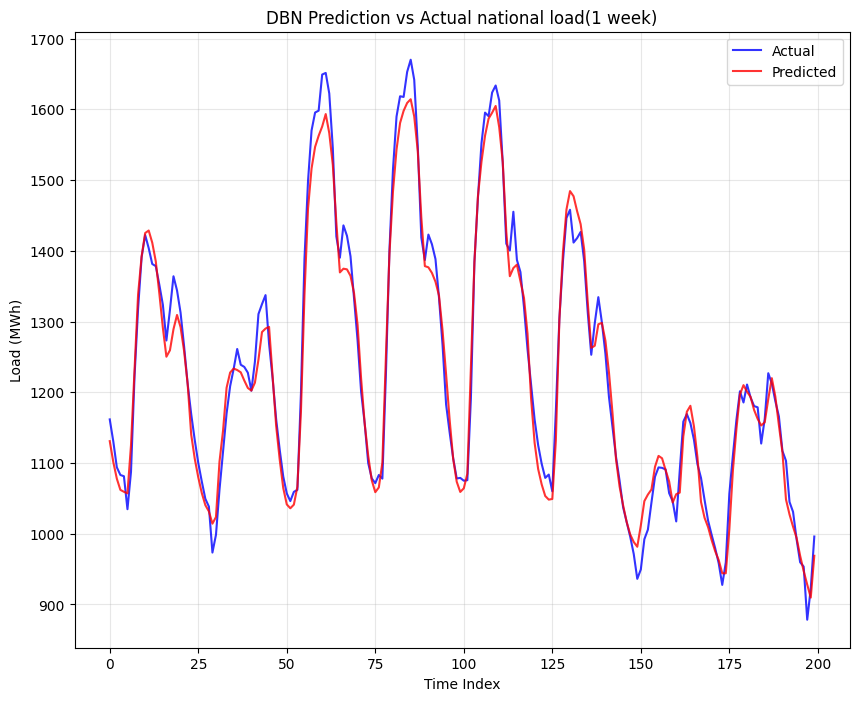
\includegraphics[width=\linewidth]{Chapters/images/results/DBN_predicted_vs_actual}
  		\caption{Predicted vs Actual load over a 1 week period of DBN}
  		\label{fig:dbnpredictedvsactual}
  	\end{minipage}
  	\hfill
  	\begin{minipage}[b]{0.48\linewidth}
  		\centering
  		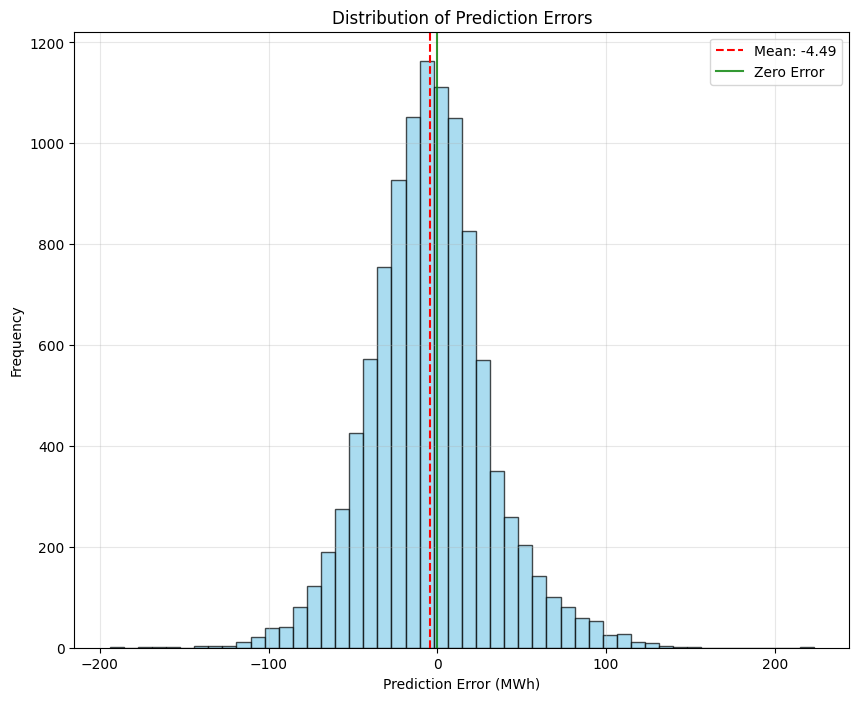
\includegraphics[width=\linewidth]{Chapters/images/results/dbn_error_distribution}
  		\caption{Distribution of prediction errors for the DBN model}
  		\label{fig:dbnerrordistribution}
  	\end{minipage}
  \end{figure}
  
  Figure \ref{fig:dbnpredictedvsactual} illustrates how the predicted load closely follows the actual load over a one-week period. The model’s errors are minimal, as highlighted in Figure \ref{fig:dbnerrordistribution}, which shows the distribution of prediction errors across all test cases. The error distribution approximates a normal distribution, with the majority of errors clustered near zero, indicating strong predictive performance.   
  \begin{figure}[h]
  	\centering
  	\includegraphics[width=0.5\linewidth]{"Chapters/images/results/dbn_validation loss"}
  	\caption{DBN model loss during training and validation}
  	\label{fig:dbnvalidation-loss}
  \end{figure}
 
 
 \subsection{CNN model results}
 
 The CNN model produced a Test MAPE of 2.74 however similar to the DBN values, with an $R^2$ value of 0.93. Table \ref{tab:cnn_performance_diff} contains the test and train results of the model. The comparison is meant to show if there was a possibility of an overfitting of the data.
 \begin{table}[h]
 	\centering
 	\caption{Performance Metrics of the CNN Model}
 	\label{tab:cnn_performance_diff}
 	\begin{tabular}{lccc}
 		\hline
 		\textbf{Metric} & \textbf{Training} & \textbf{Test} & \textbf{Difference} \\
 		\hline
 		MAPE (\%) & 1.4700 & 2.7414 & +1.2714 \\
 		MAE (Mwh) & 16.7129 & 33.0764 & +16.3635 \\
 		RMSE (Mwh) & 25.2818 & 46.8295 & +21.5477 \\
 		R$^2$ & 0.9827 & 0.9375 & -0.0452 \\
 		MSE & 639.1704 & 2192.9995 & +1553.8291 \\
 		\hline
 	\end{tabular}
 \end{table}
Similar to the results obtained for the DBN model (Section \ref{sec:dbn results}), the high $R^2$ values observed in the CNN model do not necessarily indicate overfitting. The elevated $R^2$ can be attributed to the inclusion of additional features generated during data preprocessing and feature engineering. As noted by Plevris et al. \cite{plevris2022investigation}, the $R^2$ value tends to increase with the addition of more features, even when some of these features do not have a direct correlation with the model’s output. Figure \ref{fig:cnnmodelloss} shows how the train and value loss change over the epochs. The image shows a smooth decline in the train loss, however the validation loss has a fluctuating loss that does not converge.
Figure \ref{fig:cnnpredictionvsactual} shows the prediction vs the actual output of the CNN model. The predicted load closely follows the actual load.
\begin{figure}[h]
	\centering
	\begin{minipage}[b]{0.46\linewidth}
	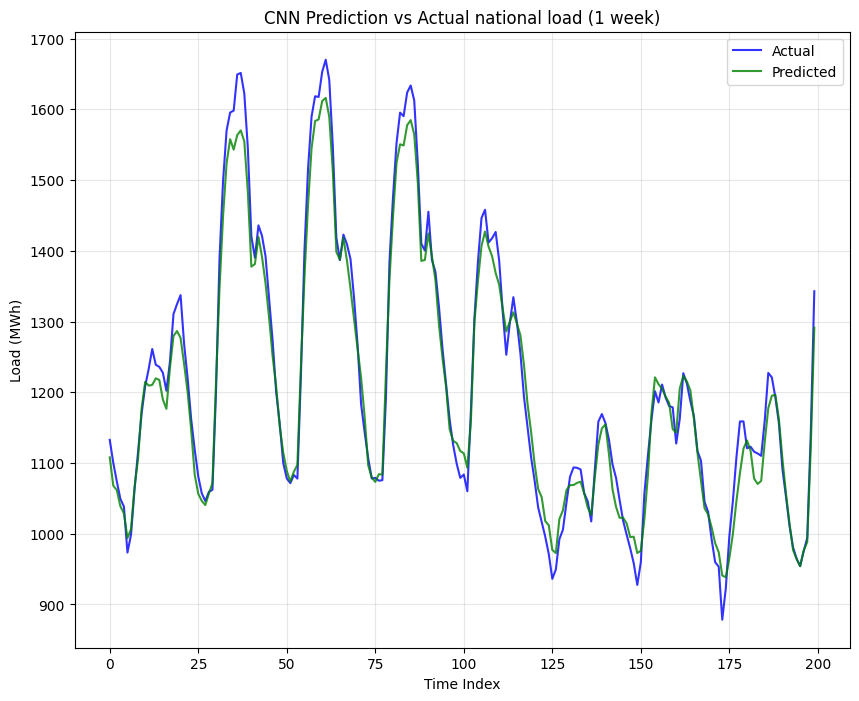
\includegraphics[width=\linewidth]{Chapters/images/results/cnn_predictionvsactual}
	\caption{The predicted and actual loading from the CNN model}
	\label{fig:cnnpredictionvsactual}
	\end{minipage}
	\begin{minipage}[b]{0.46\linewidth}
	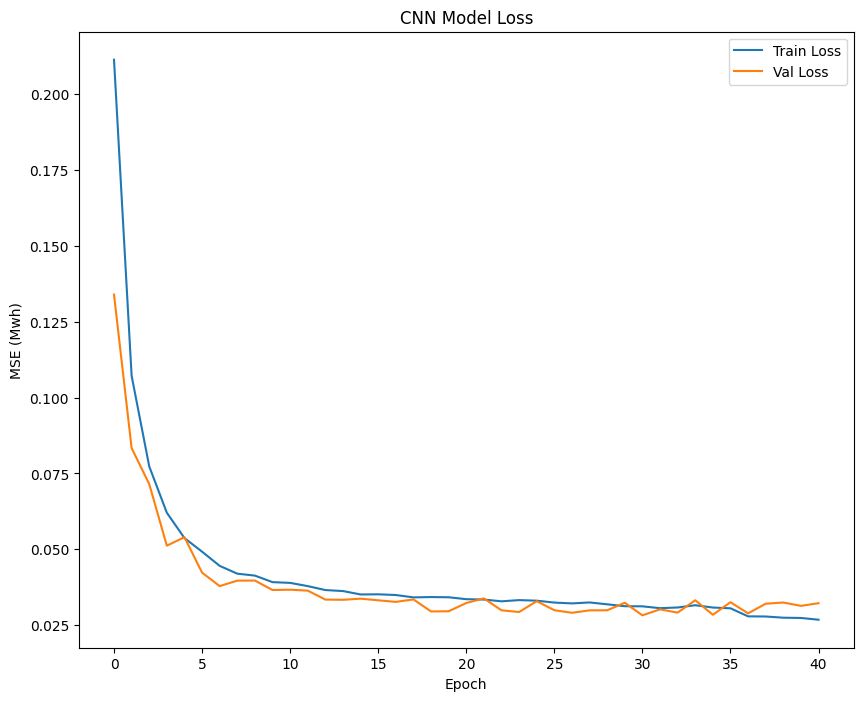
\includegraphics[width=\linewidth]{Chapters/images/results/CNN_model_loss}
	\caption{The CNN model validation and test loss against the epochs}
	\label{fig:cnnmodelloss}
	\end{minipage}
\end{figure}

\subsection{Hybrid Model Results: CNN LSTM}
 The hybrid model produced 
 \[
 b_t = \gamma (S_t - S_{t-1}) + (1-\gamma) b_{t-1}
 \tag{13}
 \label{eqn:877}
 \]


